%%%%%%%%%%%%%%%%%%%%%%%%%%%%%%%%%%%%%%%%%%%%%%%%%%%%%%%%%%%%%%%%%%%%%%%%
% Plantilla TFG/TFM
% Escuela Politécnica Superior de la Universidad de Alicante
% Realizado por: Jose Manuel Requena Plens
% Contacto: info@jmrplens.com / Telegram:@jmrplens
%%%%%%%%%%%%%%%%%%%%%%%%%%%%%%%%%%%%%%%%%%%%%%%%%%%%%%%%%%%%%%%%%%%%%%%%

\chapter{Data Generation and Semantic Segmentation}
\label{desarrollo}
\textit{This chapter develops the main work of this thesis and is organized as follows. Section \ref{sec:expanding} describes the process of automating the UnrealROX Actor. Section \ref{sec:tracker} goes through the process of recording sequences. Finally, Section \ref{sec:segnet} covers the deep learning work such as the network implementation and the data pre-processing.  }

\section{Expanding the UnrealROX Framework}
\label{sec:expanding}
As we previously mentioned in Chapter \ref{introduction}, one of the main goals of this work is to expand the UnrealROX framework in order to automatize the generation of synthetic data without the need of a VR Headset and user input. In this section we further detail the framework itself along with the data generation process.

UnrealROX can automatically generate and annotate data from a recorded sequence, but manually recording can be tedious and time consuming. In this work we have built the basic framework for the programmer to include their own actions and execute them in a sequential way, much like other frameworks such as VirtualHome by \cite{virtualhome2018}. 

\subsection{The ROXBasePawn Class}
This is the main class that contains all the logic for the character controller (movement, animations, grasping) of any robot pawn. It allows for the user to introduce a robot to the scene and manually move and interact with the objects in a scene. We use this as our parent class for the implementation.

\subsection{The ROXBotPawn Class}
The ROXBotPawn class inherits from ROXBasePawn and handles all the logic for the automation of tasks of any \textit{Actor} within a scene. In order to model all the different actions and interactions, the Enum $EActionType$ was created, where the programmer can add any type of action to be built into the system.

Also, in order to model the actions themselves, the $FROXAction$ struct was built, containing a pointer to the target, as well as the type of action $EActionType$. This structure is shown in Listing \ref{code:actionStruct}.

\begin{lstlisting}[style=C++, caption=FROXAction struct, frame=single, label=code:actionStruct]
	USTRUCT(BlueprintType)
	struct FROXAction
	{
		GENERATED_USTRUCT_BODY()
		UPROPERTY(BlueprintReadWrite, EditAnywhere, Category = Pathfinding)
		AActor* target;
		
		UPROPERTY(BlueprintReadWrite, EditAnywhere, Category = Pathfinding)
		EActionType action;
		
		FROXAction() : target(nullptr), action(EActionType::MoveTo) {};
		FROXAction(AActor* tg, EActionType t) : target(tg), action(t) {};
	}
\end{lstlisting}

In order for the programmer to add actions and queue them from the \gls{ue4}, editor we built the $doAction(AActor*, EActionType)$ (seen in Listing \ref{code:queueAction}) and made it BlueprintCallable, this way, in a simple manner, actions can be queued from the editor and the $Pawn$ will execute them in a sequential order as seen in Figure \ref{action_queue}. The target actor can be picked from the editor by creating a new variable and the type of action can be selected with a drop-down menu in the body of the blueprint function.

\begin{lstlisting}[style=C++, caption=doAction function which queues a new FROXAction to the system, frame=single, label=code:queueAction]
	UFUNCTION(BlueprintCallable)
	void AROXBotPawn::doAction(AActor* actor, EActionType type) 
	{	
		actions.Add(FROXAction(actor, type));
	}
\end{lstlisting}

\begin{figure}[!ht]
	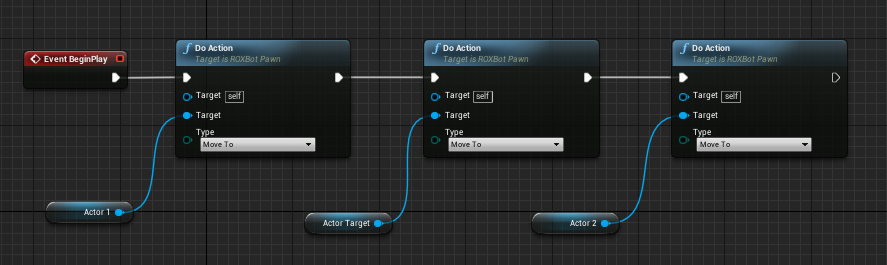
\includegraphics[scale=0.4]{archivos/action_queue.png}
	\centering
	\caption{Example of queuing 3 "MoveTo" actions from the editor}
	\label{action_queue}
\end{figure}

The $doAction()$ method creates a $FROXActions$ and pushes it to the queue. Whenever the queue contains an action and the $Pawn$ is not executing one, it will run the $fetchNextAction()$ method. This will pop the action from the queue and execute the method corresponding to that action.

Additionally, pathfinding and movement logic was implemented in order to define the $MoveTo$ action. In a first approach, the MoveToLocation method of the default \gls{ue4} Actor class was used, but the idea was discarded since we needed to work with the ROXBasePawn instead of the default Actor. Another option that was studied was Environment Query Systems (EQS), which is an experimental feature within the \gls{ai} system in \gls{ue4} which allows to gather data from the environment, e.g., the distance from one object to another or whether they are in line of sight or not. With this data we can perform queries and move accordingly to our goal, however, this method was finally discarded since the complexity of the technology was greater than that of the task we needed to solve. This is due to the fact that we only need the position of a certain actor in order to travel towards them, and this can be achieved without the need of more complex objects. 

With the previous options discarded, we decided to go with a custom implementation of the movement. In order to accomplish this, the NavigationMesh component of \gls{ue4} was used along with the $FindPathToActorSynchronously$ method, which returns a $UNavigationPath$ containing all the path-points from one actor to another. Once we obtain the path-points the $VInterpConstantTo$ from the FMath library and the $RInterpTo\_Constant$ from the UKismeMathLibrary are used in order to obtain the next vector transformation for both position and rotation of the $Pawn$, this movement logic can be seen in Listing \ref{code:movementLogic}. These methods interpolate the current location with the next path-point location in order to achieve a smooth transition and make the movement more natural.

\begin{lstlisting}[style=C++, caption=Movement logic for the pathfinding algorithm, frame=single, label=code:movementLogic]
	FVector nextPos = FMath::VInterpConstantTo(this->ActorLocation(), FVector(pathPoints[i].X, pathPoints[i].Y, ActorLocation().Z), DeltaTime, vel);
	FRotator nextRot = UKismetMathLibrary::RInterpTo_Constant(ActorRotation(), UKismetMathLibrary::FindLookAtRotation(ActorLocation(), nextPos), DeltaTime, rotateVel);
	SetActorRotation(nextRot);
	SetActorLocation(nextPos);
\end{lstlisting}

\subsection{Animating the ROXBotPawn}
As we previously mentioned in Section \ref{sec:sim2real}, simulating the 3D environment with extreme detail is a must in order for \gls{dl} algorithms to properly infer the knowledge and transfer it to the real world. In this section we take a look into the process of creating a new animation for the ROXBotPawn using \gls{ue4} blueprints.

The ROXBasePawn already provides a default walking animation for our Actor, however it is thought to work with a VR Headset, therefore, it takes into account the pose and movement of both hand controllers and the headset itself in order to move accordingly to the user. Since our ROXBotPawn does not require such data, we will change the blueprint animation in order to fit our needs. 

First of all, we need animation assets, in our case we will be using the default walk and idle animation from the UnrealROX framework since they fit our needs. In order to have smooth transitions between different animations, e.g., from idle to walking, we have used \gls{ue4} BlendSpaces, which are special assets that can be sampled in the Animation Graph and allow for blended transitions based on one or more inputs. In our case,  we will blend the animation based on the speed of the Bot, a preview of said asset can be seen in Figure \ref{fig:blend_space}.

\begin{figure}[h]
	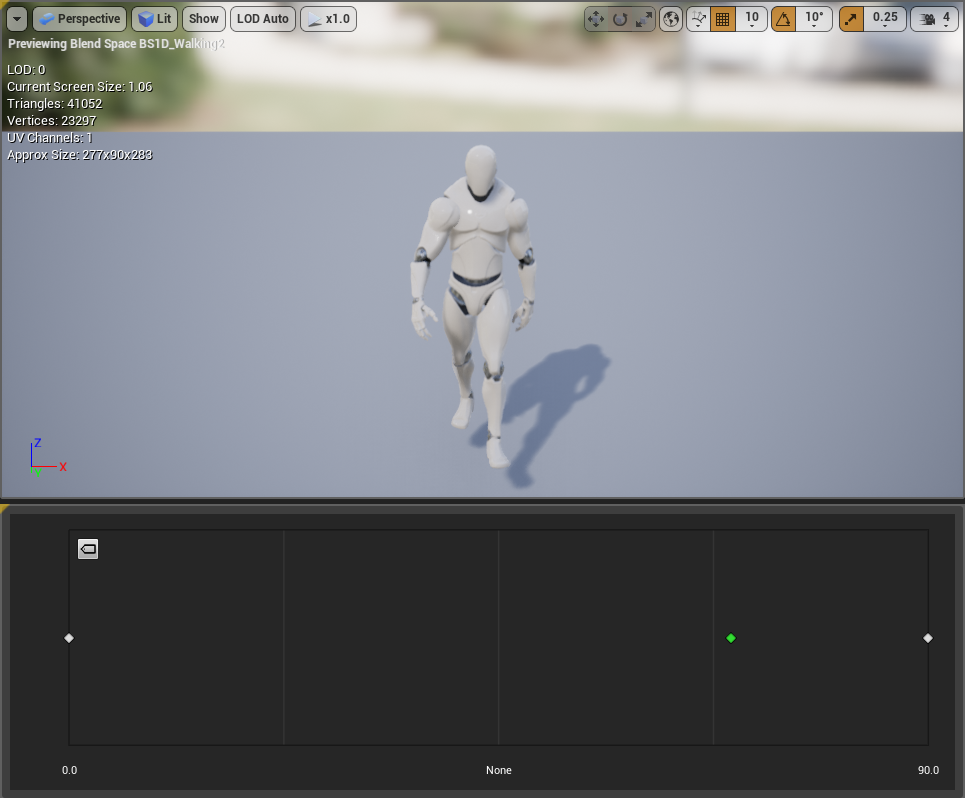
\includegraphics[width=0.5\textwidth]{archivos/blend_space.png}
	\centering
	\caption{Blend Space asset which samples the transition from idle walking state animation, 0 speed would translate into a complete idle, while 90 would be walking forward.}
	\label{fig:blend_space}
\end{figure}

In order to use the BlendSpaces, we need to create our Event Graph and compute the Bot speed, we do this by obtaining its position in the current and last tick, therefore obtaining the travel distance in one tick. We can now apply the dot operator with the forward vector and divide by the delta time, obtaining the current speed. The complete logic of this function as well as the full Event Graph can be seen in Figure \ref{fig:event_graph}.

\begin{figure}[!ht]
	\centering
	\begin{subfigure}[b]{0.8\textwidth}
		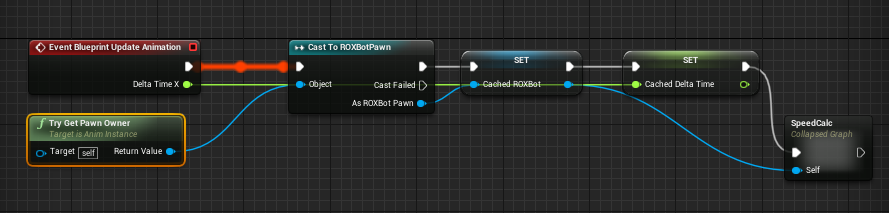
\includegraphics[width=1\linewidth]{archivos/animation_event_graph.png}
		\caption{Animation event graph.}
	\end{subfigure}
	
	\begin{subfigure}[b]{0.8\textwidth}
		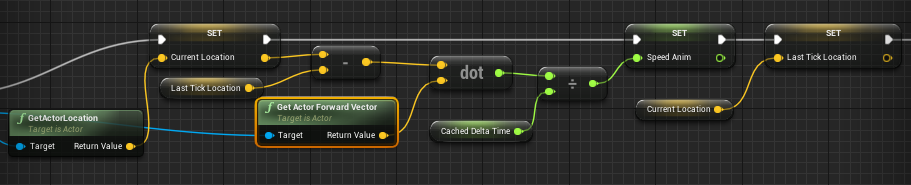
\includegraphics[width=1\linewidth]{archivos/speed_calc.png}
		\caption{SpeedCalc sub-module.}
	\end{subfigure}
	
	\caption{a) Event graph that obtains the data of the Bot. b) Blueprint sub-module which computes the instantaneous speed of the Bot.}
	\label{fig:event_graph}
\end{figure}

With the event graph and the BlendSpaces created, all there is left to do is to create the state machine, which contains the state and transition logic of the different animations. In our case, we just need an idle, walk forward and walk backwards states. This state machine is shown in Figure \ref{fig:state_machine}.

\begin{figure}[!ht]
	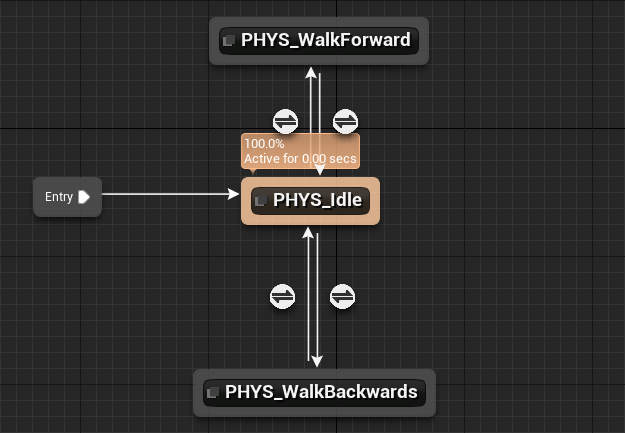
\includegraphics[scale=0.6]{archivos/animation_state_machine.png}
	\centering
	\caption{Animation state machine with idle, walk forward and walk backwards states and the transitions logic.}
	\label{fig:state_machine}
\end{figure}

The logic for the transitions between states is implemented by checking whether the speed surpasses a certain threshold, for instance, if the $Speed Anim$ is greater than 0.1, we will transition from the $Idle$ state to the $WalkForward$, in the same manner, when the speed value falls under negative $0.1$, we will transition towards the $WalkBackwards$ state.

\section{Recording sequences with UnrealROX}
\label{sec:tracker}
In this section we go through the ROXTracker class and how to use it in order to record sequences (Subsection \ref{sec:recording}) as well as how to play them and generate the data (Subsection \ref{sec:playback}).

The ROXTracker is an empty $Actor$ which means that it has no mesh or physical appearance in the world. However, this actor has knowledge of the whole scene and is able to determine the pose, rotation and materials of every other $Actor$ of the scene. In order to use it, we just need to search for it in the contextual menu (as shown in Figure \ref{fig:tracker_object}) and drag it into our scene. While in record mode, the ROXTracker is be able to store all of the information needed in order to rebuild the sequence as a TXT or JSON file. This information is then parsed in order to run the sequence in playback mode. While the sequence is being reproduced, the ROXTracker generates frame by frame the ground truth annotated images such as the segmentation masks, depth and normal maps.

\begin{figure}[h]
	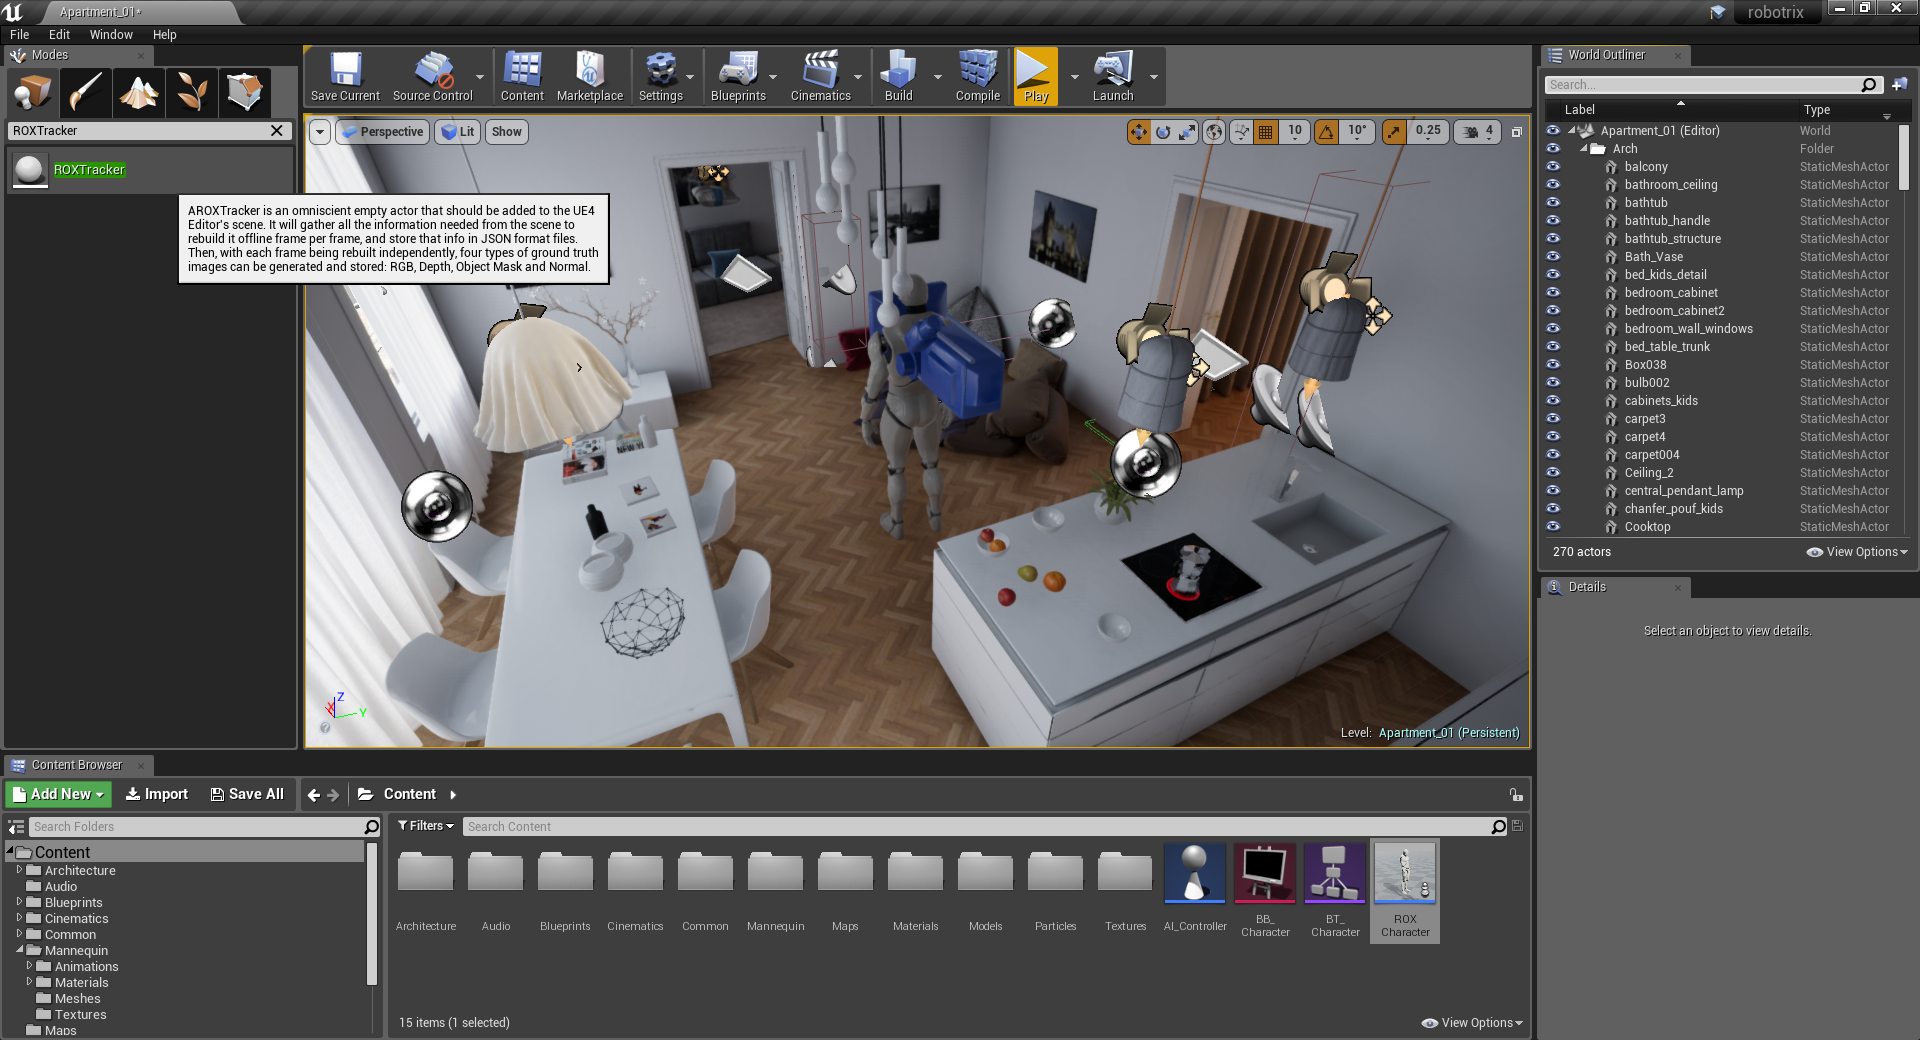
\includegraphics[width=\textwidth]{archivos/tracker_object.png}
	\centering
	\caption{ROXTracker Object in the \gls{ue4} contextual menu.}
	\label{fig:tracker_object}
\end{figure}

Once we have our ROXTracker in the World Outliner, we can tweak its behavior and change certain settings, some of the most important ones are listed as follows:

\begin{itemize}
	\item \textbf{Record Mode:} When checked, the ROXTracker will operate in record mode, this means that if the user presses the record key, it will start gathering and writing all of the necessary data to a TXT file.
	\item \textbf{Scene Save Directory:} As its own name implies, this variable stores the path where the data will be saved.
	\item \textbf{Scene Folder:}  Name of the folder inside the Scene Save Directory path where all the data files will be stored.
	\item \textbf{Generate Sequence Json:} When pressed, will look for a TXT file inside the Scene Folder with a name corresponding to the field \textbf{Input Scene TXT File Name}. Then it will generate its equivalent JSON file with the name on the field \textbf{Output Scene Json File Name}. In other words, looking at Figure \ref{fig:tracker_settings}, the Tracker will search for a $scene.txt$ file inside the $unrealrox/RecordedSequences$ folder and generate a $scene.json$ file.
\end{itemize}

\begin{figure}[!ht]
	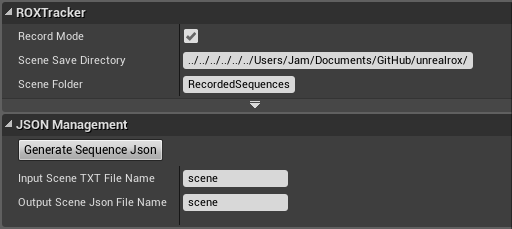
\includegraphics[width=0.8\textwidth]{archivos/tracker_settings.png}
	\centering
	\caption{ROXTracker settings in the \gls{ue4} editor.}
	\label{fig:tracker_settings}
\end{figure}

\subsection{Recording mode}
\label{sec:recording}

Before we start generating sequences, we need to make some tweaks to the recording settings of the ROXTracker, which can be seen in Figure \ref{fig:recording_settings} and further explained as follows:

\begin{itemize}
	\item \textbf{Pawns:} Array that contains a reference to every actor that the user wants to keep track of.
	\item \textbf{Camera Actors:} Array containing the cameras that will be tracked.
	\item \textbf{Stereo Camera Baselines:} Array that stores the focal distance (baseline) between the corresponding camera in the \textbf{CameraActors} array. It can be left empty if there are none.
	\item \textbf{Scene File Name Prefix:} Every generated file of raw scene data will share this prefix in its filename.
\end{itemize}

\begin{figure}[!ht]
	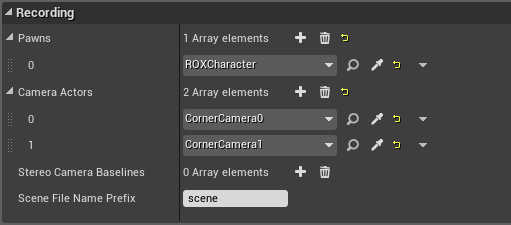
\includegraphics[width=0.5\textwidth]{archivos/recording_settings.png}
	\centering
	\caption{ROXTracker recording settings.}
	\label{fig:recording_settings}
\end{figure}

Once all of the fields are filled with the desired actors and cameras to be tracked and the filenames are set, we can start recording a sequence, to do this, we simply have to set the ROXTracker in record mode and run the scene by hitting play on the editor. To begin or stop the recording, the user needs to press "R", a red \textbf{RECORDING} message will then be displayed at the top of the screen. An example of the recorder running can be seen in Figure \ref{fig:recording}.

\begin{figure}[!ht]
	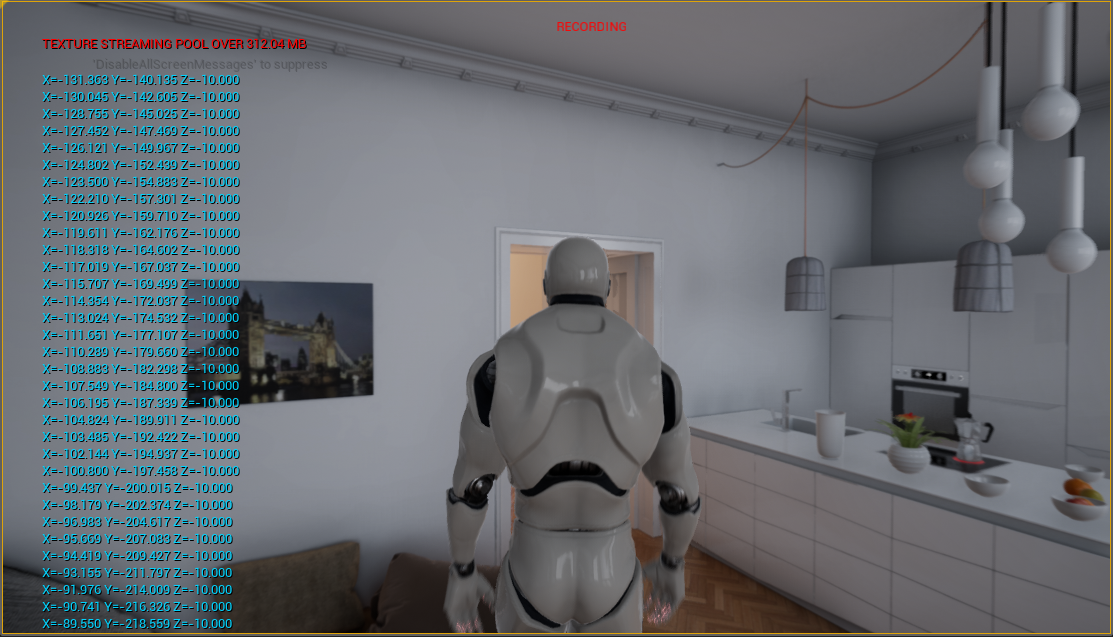
\includegraphics[width=0.6\textwidth]{archivos/recording.png}
	\centering
	\caption{Example of a running scene being recorded.}
	\label{fig:recording}
\end{figure}

When the sequence finishes, we can stop recording. If we take a look at our designated Scene Folder for the data generation, we can see our raw recording data in TXT format. We now need, in order to get it ready for playback, to parse it to JSON, we can do this with the \textbf{Generate Sequence Json} utility displayed in Figure \ref{fig:tracker_settings}.

\subsection{Playback mode}
\label{sec:playback}
Before we are able to play the sequences in the \gls{ue4} editor, we have to go through some of the configuration settings for the playback mode, which can be seen in Figure \ref{fig:playback_settings} and are further explained below:

\begin{itemize}
	\item \textbf{Json File Names:} Array containing all the JSON filenames that we want to playback.
	\item \textbf{Start Frames:} Array that contains the starting frames for each JSON. The index in this array will directly correlate to the one in the \textbf{Json File Names} array.
	\item \textbf{Playback Only:} When active, it will only play the sequence, skipping the data generation process.
	\item \textbf{Playback Speed Rate:} As its own name indicates, allows to set the speed of the playback, although it can only be used in \textbf{Playback Only} mode. 
	\item \textbf{Generate RGB, Depth, Object Mask, Normal:} It will generate the RGB (format can be adjusted in the \textbf{Format RGB} option), Depth, Segmentation Masks and Normal maps for each frame and camera.
	\item \textbf{Generate Depth Txt Cm:} Generates an equivalent TXT file to the Depth image, where the depth values are stored as plain text.
	\item \textbf{Screenshot Save Directory:} Base path where the Screenshot folder will be located.
	\item \textbf{Screenshot Folder:} Name of the folder where the screenshots will be saved.
	\item \textbf{Width/Height:} Output resolution of the generated images.
\end{itemize}

\begin{figure}[h]
	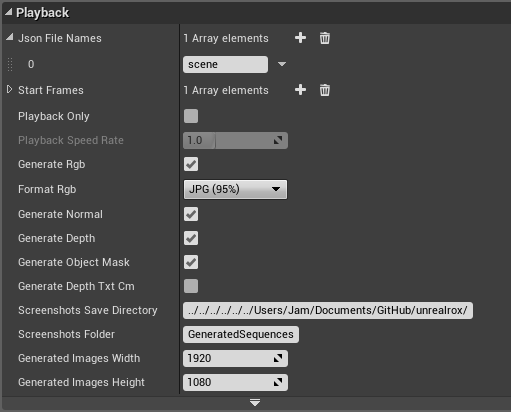
\includegraphics[width=0.5\textwidth]{archivos/playback_settings.png}
	\centering
	\caption{ROXTracker playback settings.}
	\label{fig:playback_settings}
\end{figure}

Once the desired configuration is set and the Record Mode is disabled, we can press play in the editor. The ROXTracker object will start parsing the sequence JSON file and generating the output images in our designated folder, an example of the four different outputs is shown in Figure \ref{fig:playback_output}.

\begin{figure*}[!ht]
	\centering
	\begin{subfigure}[b]{0.475\textwidth}
		\centering
		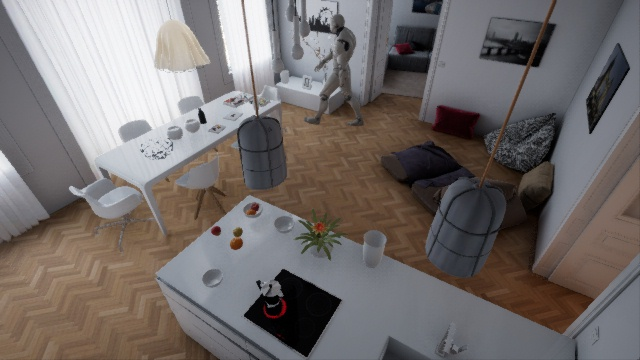
\includegraphics[width=\textwidth]{archivos/generated_rgb.jpg}
		\caption[Output RGB image.]%
		{{\small Output RGB image.}}    
		\label{fig:generated_rgb}
	\end{subfigure}
	\hfill
	\begin{subfigure}[b]{0.475\textwidth}  
		\centering 
		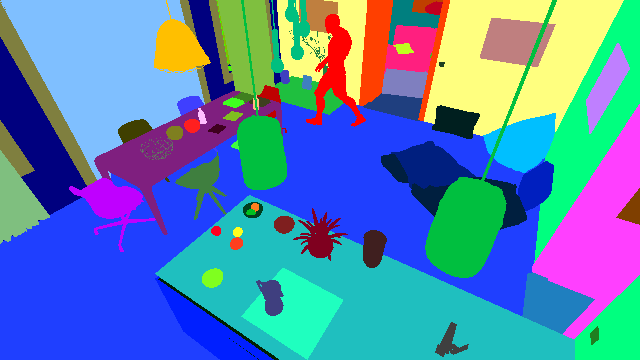
\includegraphics[width=\textwidth]{archivos/generated_mask.png}
		\caption[Output Segmentation Masks.]%
		{{\small Output Segmentation Masks.}}    
		\label{fig:generated_mask}
	\end{subfigure}
	\vskip\baselineskip
	\begin{subfigure}[b]{0.475\textwidth}   
		\centering 
		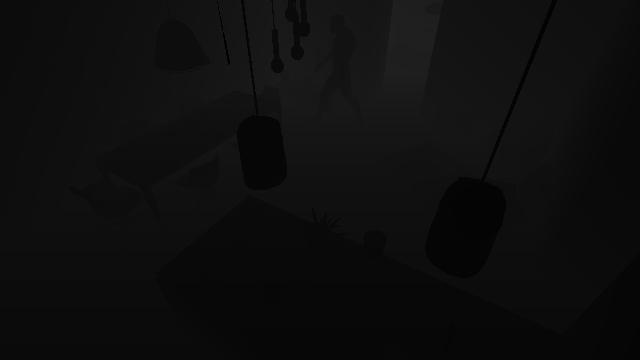
\includegraphics[width=\textwidth]{archivos/generated_depth.png}
		\caption[Output Depth image.]%
		{{\small Output Depth image.}}    
		\label{fig:generated_depth}
	\end{subfigure}
	\quad
	\begin{subfigure}[b]{0.475\textwidth}   
		\centering 
		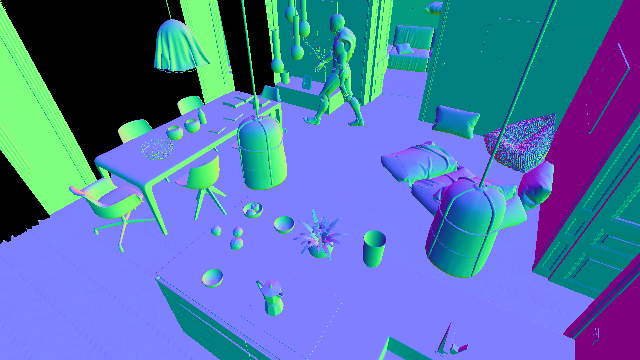
\includegraphics[width=\textwidth]{archivos/generated_normals.png}
		\caption[Output Normals image.]%
		{{\small Output Normals image.}}    
		\label{fig:generated_normals}
	\end{subfigure}
	\caption{Output examples of the Tracker in playback mode.}
	\label{fig:playback_output}
\end{figure*}

\section{Implementing a SegNet using PyTorch}
\label{sec:segnet}
As we previously mentioned, one of the main goals of this work is to study how synthetic data can help semantic segmentation algorithms. For this purpose, a SegNet has been implemented and trained with a real-world human-pose dataset. This Section will cover all the data processing, as well as the design and development process of such network.

\subsection{Preprocessing the dataset}
\label{sec:preprocess}
In Section \ref{sec:datasets} we mentioned a few of the most important datasets in the field, however, all of them are general purpose oriented, and for this work we needed a human pose dataset. Because of this, we decided to use the \gls{utp} dataset by \cite{Lassner:UP:2017}. Most of the images from this dataset come from the MPII Human Pose Dataset and contains both the RGB and the Segmentation Mask image.

However, some data pre-processing will be needed in order to fit the data to our needs, this is further detailed in the following Subsections.

\subsubsection{Merging the segmentation masks}
The \gls{utp} dataset is divided by segmentation instances. This means that a full image with different persons is divided in different images, each with its unique segmentation mask. For our purpose, we wanted the full image without the instance information. The dataset provides a CSV file which contains the image ID for every segmentation instance in sequential order. This means that we can get all the instances that share the same image ID by iterating through the CSV file. Listing \ref{code:numInstances} shows how we obtain the amount of instances for a single image ID.

\begin{lstlisting}[style=Python-color, caption=Obtaining the number of instances for a single image, frame=single, label=code:numInstances]
	csv = pd.read_csv(csv_path)
	
	while x < len(csv):
		instances = 0
		
		for id in range(x, len(csv)):
			if csv['mpii_id'][id] == csv['mpii_id'][id+1]:
				instances += 1
			else:
				break
\end{lstlisting}

Having obtained the amount of instances and with our iterator $x$ pointing to the first image, we can now obtain all the following images and merge them as shown in Listing \ref{code:mergeInstances}. To do this, we use the $Paste$ method from the $Pillow$ library, which takes two inputs: the image to be pasted and the mask which contains the pixels that are to be copied into the first image. In our case, the mask already fits our purpose since it is the mask that we want to copy.

\begin{lstlisting}[style=Python-color, caption=Merging the instance masks into a single image, frame=single, label=code:mergeInstances]
	first_image = Image.open(img_path + str(x))
	
	for n in range(1, instances + 1):
		next_image = Image.open(img_path + str(x + n))
		first_image.paste(next_image, (0,0), next_image.convert('L'))
		
	new_id += 1
	x += instances + 1
\end{lstlisting}

\subsubsection{Creating the dataset class}
Before we can train our network, we need to design a data loader class that will fetch our dataset and transform the data to the proper format. For this purpose, we used the PyTorch Dataset class, which allows us to create our data loaders, this way all the data and batch processing will be handled by the framework. Listing \ref{code:UTPDataset} shows the main structure of the UTPDataset class.

\begin{lstlisting}[style=Python-color, caption=UTPDataset definition, frame=single, label=code:UTPDataset]
	class UTPDataset(Dataset):
		def __init__(self, img_dir, transform=None):
			self.transform = transform
			self.image_root_dir = img_dir
			self.img_extension = '_full.png'
			self.mask_extension = '_segmentation_full.png'
			
		def __getitem__(self, index):
			image_id = str(index).zfill(5)
			image_path = os.path.join(self.image_root_dir, image_id, self.img_extension)
			mask_path = os.path.join(self.image_root_dir, image_id, self.mask_extension)
			
			image = self.load_image(path=image_path)
			mask = self.load_mask(path=mask_path)
			
			data =  {
						'image': torch.FloatTensor(image),
						'mask' : torch.LongTensor(mask)
					}
					
			return data
			
\end{lstlisting}

The \textbf{$\_\_getitem\_\_$} method returns the rgb-mask pair when given an index. In order to load the image, we compute the filename using the $zfill$ method, this will add leading zeros to the index so it fits the image name. We then call the $load\_image$ and $load\_mask$ methods shown in Listing \ref{code:UTPload}, which loads and processes the data. Finally, we insert it into a small dictionary and return it.

\begin{lstlisting}[style=Python-color, caption=UTPDataset rgb and mask load and pre-processing, frame=single, label=code:UTPload]
	PALETTE = {
		(0,		0,		0)		:	0,		#Human
		(255,	255,	255)	:	1,		#Background
	}

	def load_image(self, path=None):
		raw_image = Image.open(path)
		raw_image = np.transpose(raw_image.resize((224,224)), (2,1,0))
		imx_t = np.array(raw_image, dtype=np.float32)/255.0
		
		return imx_t

	def load_mask(self, path=None):
		raw_image = Image.open(path)
		raw_image = raw_image.resize((224,224))
		imx_t = np.array(raw_image)
		label_seg = np.zeros((2,224,224), dtype=np.int)
		
		for k in PALETTE:
			label_seg[PALETTE[k]][(imx_t==k).all(axis=2)] = 1
		
		return label_seg
		
\end{lstlisting}

It is important to remark that the input data format for the masks is $(N \times C \times H \times W)$ where $N$ is the batch size, $C$ the number of classes and $H \times W$ the height and width of the image. The segmentation masks are one-hot encoded, which means that each class has, omitting the batch size, a $(1 \times H \times W)$ image where the pixels belonging to the $C$ class are stored as 1 and the rest as 0. The method $load\_mask$ in Listing \ref{code:UTPload} performs such encoding by iterating through all the classes stored on the $PALLETE$ dictionary, where the RGB values for each class are stored. For every class and starting with a zero-filled matrix, we write only on the pixel coordinates of the mask that corresponds to the RGB value of the current class. This encoding is depicted in Figure \ref{fig:onehot}.

\begin{figure}[!ht]
	\centering
	
	\begin{subfigure}[b]{0.7\textwidth}
		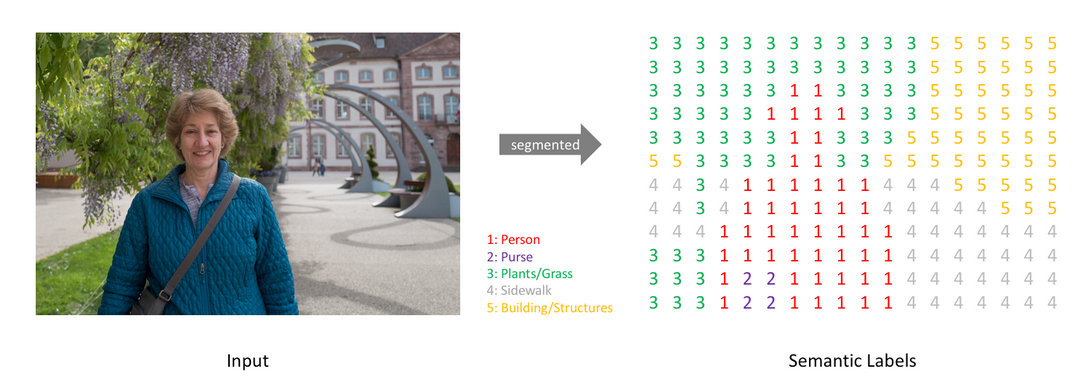
\includegraphics[width=1\linewidth]{archivos/segmentation_encoding.png}
		\caption{Regular segmentation mask codification.}
	\end{subfigure}
	
	\begin{subfigure}[b]{0.5\textwidth}
		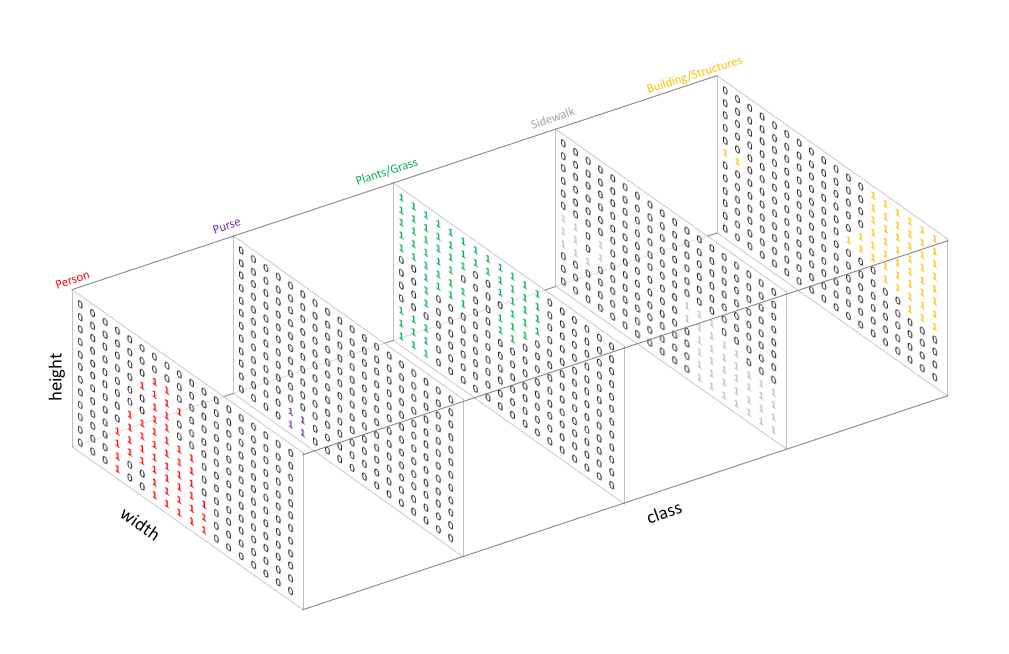
\includegraphics[width=1\linewidth]{archivos/segmentation_encoding2.png}
		\caption{One-hot encoded masks.}
	\end{subfigure}
	
	\caption[One-hot encoding format from a regular segmentation mask.]{One-hot encoding format from a regular segmentation mask. Extracted from Jeremy Jordan semantic segmentation post\footnotemark.}
	\label{fig:onehot}
\end{figure}
\footnotetext{\url{https://www.jeremyjordan.me/semantic-segmentation/}}

\subsubsection{From UnrealROX to UTP}
When loading images from the UnrealROX dataset, segmentation masks are slightly different since we have more than 30 classes. However, our network expected classes are only background and human. To overcome this problem we built two different scripts. The first one is shown in Listing \ref{code:rox-onehot} and its purpose is to encode the segmentation masks so that it only contains the human and background class. 

\begin{lstlisting}[style=Python-color, caption=Preprocessing the UnrealROX segmentation masks, frame=single, label=code:rox-onehot]
imx_t = np.array(raw_image)
imx_t = imx_t[:,:,:3]
label_seg = np.zeros((2,224,224), dtype=np.int)

label_seg[0][(imx_t==[255,0,0]).all(axis=2)] = 1
label_seg[1][np.where(label_seg[0] == 0)] = 1

\end{lstlisting}

It works in a similar manner to the one-hot encoding on the $load\_mask$ method (Listing \ref{code:UTPload}). In the same fashion, we create a $(2 \times H \times W)$ zero-filled array. Then for the first layer we fill with ones the [255,0,0] RGB value since it corresponds to the human class, as for the second layer, we simply invert the first in order to obtain the background. The result can be seen in Figure \ref{fig:rox-onehot}.

\begin{figure}[!ht]
	\centering
	\begin{subfigure}[b]{0.4\textwidth}
		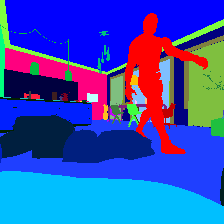
\includegraphics[width=1\linewidth]{archivos/rox_mask.png}
		\caption{Sample UnrealROX segmentation mask.}
	\end{subfigure}
	
	\begin{subfigure}[b]{0.6\textwidth}
		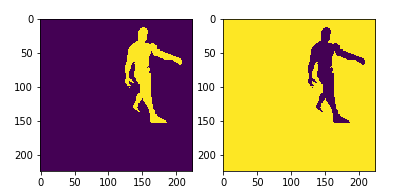
\includegraphics[width=1\linewidth]{archivos/onehot_mask.png}
		\caption{One-hot two-class segmentation mask.}
	\end{subfigure}
	
	\caption{UnrealROX segmentation masks before and after the pre-process pass.}
	\label{fig:rox-onehot}
\end{figure}

The second script is shown in Listing \ref{code:rox-to-utp}. Its main purpose is to adapt the data generated with UnrealROX to the \gls{utp} format, in such a way that the \gls{utp} dataset class can process the ROX data without extra logic. In order to do this, we iterate through the directory structure of the generated data (Figure \ref{fig:rox-dir}), process each image and move them to our \gls{utp} dataset folder. The outermost for loop will iterate through the cameras of the scene. For each camera, we iterate through all the images in both the $rgb$ and $mask$ folders. The RGB images are simply renamed and moved to the dataset folder, however, the segmentation masks require some pre-processing. As seen in the previous script, we need to get rid of the unnecessary classes. This time, we want the image in the \gls{utp} RGB format, which is [255,255,255] for the person class, and [0,0,0] for the background class. Listing \ref{code:process_mask} shows the $process\_mask$ method which performs such processing.

\begin{lstlisting}[style=Python-color, caption=UnrealROX data to UTP format, frame=single, label=code:rox-to-utp]
directory = 'scene1/'
dataset_path = 'dataset/dataset/'

new_id = len(os.listdir(dataset_path)) // 2

for camera in ['CornerCamera0/', 'CornerCamera1/', 'MainCamera/']:
	for idx in range(1,len(os.listdir(os.path.join(directory, 'rgb', camera)))):
		if idx % 10 == 0:
			filename = str(idx).zfill(6) + '.png'
			os.rename(directory + 'rgb/' + camera + filename, dataset_path + str(new_id).zfill(5) + '_full.png')
			
			raw_image = Image.open(directory + 'mask/' + camera + filename)
			raw_image = raw_image.convert('RGB')	
			raw_image = process_mask(raw_image)

			raw_image.save(dataset_path + str(new_id).zfill(5) + '_segmentation_full.png')
			new_id += 1

\end{lstlisting}

\begin{lstlisting}[style=Python-color, caption=process\_mask method whithin the script, frame=single, label=code:process_mask]
pixels = raw_image.load()
for i in range(raw_image.size[0]):
	for j in range(raw_image.size[1]):
		if pixels[i,j] == (255, 0, 0):
			raw_image.putpixel((i,j), (255, 255, 255))
		else:
			raw_image.putpixel((i,j), (0, 0, 0))

\end{lstlisting}

\begin{figure}[!ht]
	\centering
	\begin{forest}
		for tree={
			font=\ttfamily,
			grow'=0,
			child anchor=west,
			parent anchor=south,
			anchor=west,
			calign=first,
			edge path={
				\noexpand\path [draw, \forestoption{edge}]
				(!u.south west) +(7.5pt,0) |- node[fill,inner sep=1.25pt] {} (.child anchor)\forestoption{edge label};
			},
			before typesetting nodes={
				if n=1
				{insert before={[,phantom]}}
				{}
			},
			fit=band,
			before computing xy={l=15pt},
		}
		[Scene1
		[rgb
		[Camera1]
		[Camera2]
		[...]
		]
		[mask
		[Camera1]
		[Camera2]
		[...]
		]
		]
	\end{forest}
	\caption{Directory structure of the generated UnrealROX data.}
	\label{fig:rox-dir}
\end{figure}

\subsection{Training the network}
\label{sec:training}
In this Subsection we go through the network implementation and the training script.

\subsubsection{SegNet Model}
\label{sec:model}
In Section \ref{sec:segmentation_variants} we described the encoder-decoder variant used on \gls{cnn}s for semantic segmentation, specifically, we described the SegNet architecture. This Subsection describes the model implementation we used\footnote{\url{https://github.com/Sayan98/pytorch-segnet/blob/master/src/model.py}} for this work.

\begin{figure}[h]
	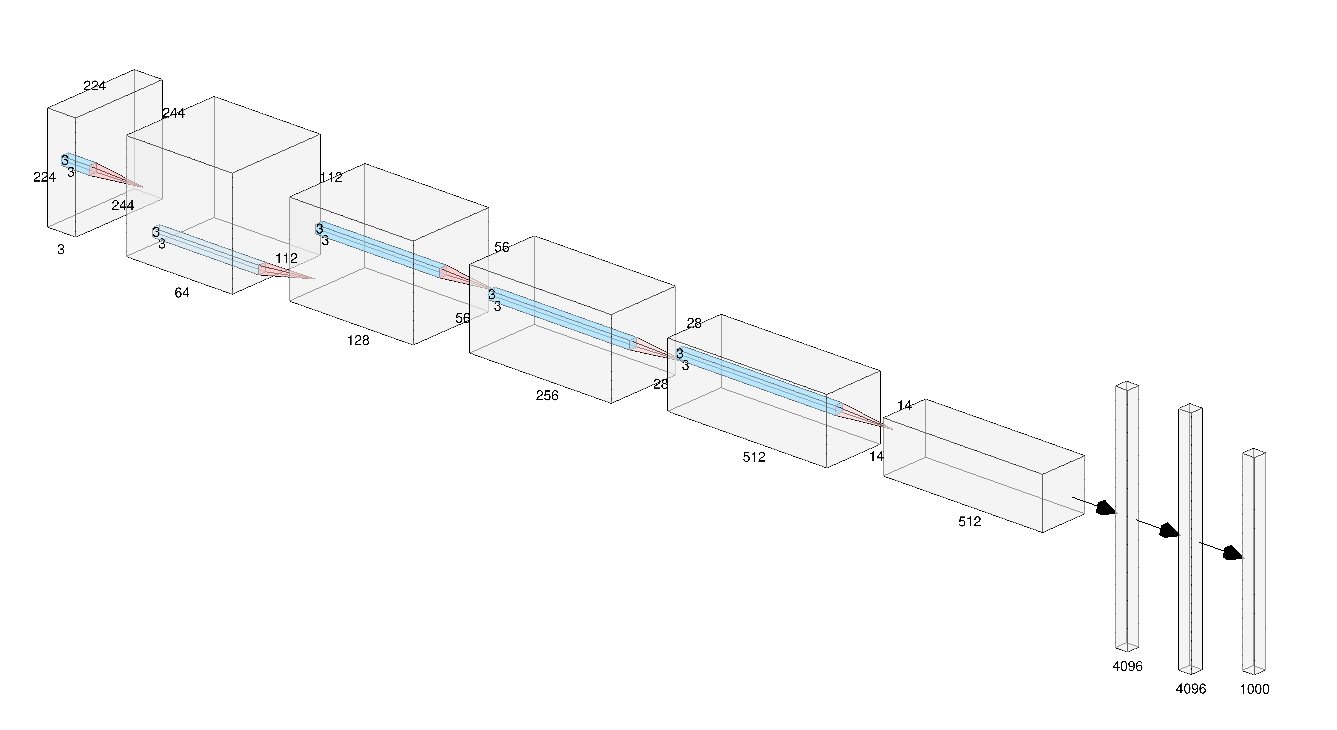
\includegraphics[width=0.6\textwidth]{archivos/vgg16.png}
	\centering
	\caption{Illustration of the VGG-16 architecture.}
	\label{fig:vgg16}
\end{figure}

The encoder and decoder layout equivalent in PyTorch is shown in Listings \ref{code:encoder} and \ref{code:decoder}. The encoder fundamentally consists of stacked convolutional layers. At the decoder, the convolutions are replaced with \textit{Convolutional Transposed Layers}, which applies a transposed convolution that upsamples the output. Additionally, every convolutional layer is followed by a batch normalization one. These layers standardize their inputs, in a way that for each mini-batch, their mean is 0 and their variance is 1. This can have slight regularization effects and can help to increase the learning process.


\begin{lstlisting}[style=Python-color, caption=First layers of the SegNet encoder, frame=single, label=code:encoder]
self.encoder_conv_00 = nn.Sequential(*[nn.Conv2d(in_channels=self.input_channels, out_channels=64, kernel_size=3, padding=1), nn.BatchNorm2d(64) ])

self.encoder_conv_01 = nn.Sequential(*[ nn.Conv2d(in_channels=64, out_channels=64, kernel_size=3, padding=1), nn.BatchNorm2d(64)])

...

self.encoder_conv_42 = nn.Sequential(*[nn.Conv2d(in_channels=512, out_channels=512, kernel_size=3, padding=1), nn.BatchNorm2d(512)])
\end{lstlisting}

\begin{lstlisting}[style=Python-color, caption=First layers of the SegNet decoder, frame=single, label=code:decoder]
self.decoder_convtr_42 = nn.Sequential(*[nn.ConvTranspose2d(in_channels=512, out_channels=512, kernel_size=3, padding=1), nn.BatchNorm2d(512)])

self.decoder_convtr_41 = nn.Sequential(*[nn.ConvTranspose2d(in_channels=512, out_channels=512, kernel_size=3, padding=1), nn.BatchNorm2d(512)])

...

self.decoder_convtr_00 = nn.Sequential(*[nn.ConvTranspose2d(in_channels=64, out_channels=self.output_channels, kernel_size=3, padding=1)])

\end{lstlisting}

Then, we need to define the forward function. This module will be perform a forward pass on the network given an input and is shown in Listings \ref{code:encoder_forward} and \ref{code:decoder_forward}. On the encoder, as with every convolutional network, we apply the activation function between layers and pooling at the end of the convolution. On the decoder, however, the order is reversed, we first apply the reverse pooling function or unpooling, then the activation functions and, finally, in the output layer, we apply a softmax classifier in order to get pixel-wise predictions.

\begin{lstlisting}[style=Python-color, caption=Forward function on the encoder, frame=single, label=code:encoder_forward]
dim_0 = input_img.size()
x_00 = F.relu(self.encoder_conv_00(input_img))
x_01 = F.relu(self.encoder_conv_01(x_00))
x_0, indices_0 = F.max_pool2d(x_01, kernel_size=2, stride=2, return_indices=True)

...

dim_4 = x_3.size()
x_40 = F.relu(self.encoder_conv_40(x_3))
x_41 = F.relu(self.encoder_conv_41(x_40))
x_42 = F.relu(self.encoder_conv_42(x_41))
x_4, indices_4 = F.max_pool2d(x_42, kernel_size=2, stride=2, return_indices=True)

\end{lstlisting}

\begin{lstlisting}[style=Python-color, caption=Forward function on the decoder, frame=single, label=code:decoder_forward]
x_4d = F.max_unpool2d(x_4, indices_4, kernel_size=2, stride=2, output_size=dim_4)
x_42d = F.relu(self.decoder_convtr_42(x_4d))
x_41d = F.relu(self.decoder_convtr_41(x_42d))
x_40d = F.relu(self.decoder_convtr_40(x_41d))
dim_4d = x_40d.size()

...

x_0d = F.max_unpool2d(x_10d, indices_0, kernel_size=2, stride=2, output_size=dim_0)
x_01d = F.relu(self.decoder_convtr_01(x_0d))
x_00d = self.decoder_convtr_00(x_01d)
dim_0d = x_00d.size()

x_softmax = F.softmax(x_00d, dim=1)

\end{lstlisting}

\subsubsection{Training script}
\label{sec:train_script}

In order to train our model, a training script was built. To do this, we create our data loaders and split the data into train and validation splits. Listing \ref{code:dataloaders} shows how the PyTorch DataLoader\footnote{\url{https://pytorch.org/docs/stable/data.html}} class can be use to create our data loaders.

When training, we can not only use the training loss as a metric for evaluation, since the network can over-fit the training samples, which means that it will not be good at generalization. Because of that, we use a split of the dataset for validation purposes.

\begin{lstlisting}[style=Python-color, caption=Data loaders and train-val split, frame=single, label=code:dataloaders]
full_dataset = UTPDataset(img_dir='dataset/dataset')

train_size = int(0.8 * len(full_dataset))
val_size = len(full_dataset) - train_size

train_dataset, val_dataset = torch.utils.data.random_split(full_dataset, [train_size, val_size])

train_dataloader = DataLoader(train_dataset, batch_size=BATCH_SIZE, shuffle=True, num_workers=6)
val_dataloader = DataLoader(val_dataset, batch_size=BATCH_SIZE, shuffle=True, num_workers=6)

data_loaders = {"train": train_dataloader, "val": val_dataloader}

\end{lstlisting}

In order to create two different data loaders for training and validation, we split the dataset with the $random\_split$ function. Then, we create the two data loaders and insert them into a dictionary, this allows us to easily differentiate the phase in every epoch.

\begin{lstlisting}[style=Python-color, caption=Model criterion and optimizer definition, frame=single, label=code:optimizer]
model = SegNet(input_channels=3, output_channels=2).cuda()
criterion = torch.nn.CrossEntropyLoss().cuda()
optimizer = torch.optim.Adam(model.parameters(), lr=LEARNING_RATE)

\end{lstlisting}

Listing \ref{code:optimizer} shows the definition of our model and the criterion, which is the metric that is used to determine how far our predictions are from the ground-truth annotation, in our case, we used Cross Entropy Loss. Finally we define our optimizer, which handles how we modify the network weights based on different criteria. In our case, we used the Adam optimizer.

With the initialization ready, we can now train the network. Algorithm \ref{alg:train} shows a high-level version of the training script. For every epoch, we process the whole dataset, which is divided in two different loaders. The $phase$ loop will determine which phase is currently being processed. Before iterating the data loaders, we need to set our model to the proper phase by using the $train()$ and $eval()$ methods. Then the inner most loop will iterate through all the batches of the loader. In this inner loop, we obtain the input RGB images and the target segmentation masks, perform the forward propagation or prediction and then compute the loss with respect to our prediction and the desired one. It is important to remark that, if we are in the training phase, we also need to compute the gradients based on our loss, as well as update the weights using our optimizer. These two steps are not needed in the validation phase since we are just doing it as a metric to know how the network is performing during training.\newline

\begin{algorithm}[!ht]
	\KwIn{model, data\_loaders, criterion}
	\KwOut{model}
	\DontPrintSemicolon
	\For{$epoch\gets0$ \KwTo $EPOCHS$}{
		\For{phase \textbf{in} ['train', 'val']}{
			$running\_loss \gets 0$\;
			\eIf{phase = 'train'}{ model.train() }{ model.eval() }
			\For{batch \textbf{in} data\_loaders[phase]}{
				$input  \gets batch['image']$\;
				$target \gets batch['mask']$\;
				
				$output \gets model(input)$\;
				$loss \gets criterion(output, target)$\;
				
				\If{phase = 'train'}{
					$loss.backward()$\;
					$optimizer.step()$\;
				}
				$running\_loss \gets running\_loss + loss$\;
			}
		}
	}
	\caption{Training script}
	\label{alg:train}
\end{algorithm}

In order to prevent our model from overfitting, model checkpoints were implemented. This method allows us to keep the best model obtained during training with respect to any measure, in our case, we kept the model with the lowest loss value on the validation set. Listing \ref{code:checkpoints} shows this implementation, where $prev\_loss$ is our best loss in the validation pass and $running\_loss$ our current validation loss. This is computed after every epoch. The $torch.save$ method persists the $mode.state\_dict()$ which is a dictionary containing the learnable parameters of the model (weights and biases).


\begin{lstlisting}[style=Python-color, caption=Model checkpoints, frame=single, label=code:checkpoints]
if running_loss < prev_loss:
	torch.save(model.state_dict(), os.path.join('.', 'epoch-{}.pth'.format(epoch+1)))
	prev_loss = running_loss

\end{lstlisting}

\subsubsection{Loading a trained model}
In order to load the model once it has been trained, PyTorch provides the $load\_state\_dict$ method. An example of its use is shown in Listing \ref{code:load_model}. It is important to note that this only works for prediction and not for training, since there are multiple parameters that are not saved on the $state\_dict$ such as the optimizer or the loss metrics. However, PyTorch does provide us with a custom $save$ method that allows to save a custom $dict$ and thus to save all the necessary parameters so that it can be used to resume training.

\begin{lstlisting}[style=Python-color, caption=Load model checkpoint, frame=single, label=code:load_model]
model = SegNet(input_channels=3, output_channels=2)
model.load_state_dict(torch.load(PATH))
model.eval()

\end{lstlisting}